\chapter{Grundlagen}
% maybe fix formating here?
 \section{Einheiten verschiedener Größen}
 \begin{minipage}{\textwidth}
   {%Workaround for evenly spaced align
    \savebox\strutbox{$\vphantom{\vec{\left[\frac{A^2}{A^2}\right]}}$}
    \begin{align}
	    \textbf{Elektrische Feldstärke }\vec{E}        & \text{ mit }\left[\vec{E}\right] =\mathrm{ \frac{V}{m} }                            \\
	    \textbf{Magnetische Feldstärke }\vec{H}        & \text{ mit }\left[\vec{H}\right]=\mathrm{ \frac{A}{m} }                             \\
	    \textbf{Elektrische Flussdichte }\vec{D}       & \text{ mit }\left[\vec{D}\right] =\mathrm{ \frac{C}{m^{2}} = \frac{A s}{m^{2}}}     \\
	    \textbf{Magnetische Flussdichte }\vec{B}       & \text{ mit }\left[\vec{B}\right] =\mathrm{ T = \frac{V s}{m^{2}} }                  \\
	    \textbf{Polarisation }\vec{P}                  & \text{ mit }\left[\vec{P}\right] = \left[\vec{D}\right] = \mathrm{\frac{C}{m^{2}} } \\
	    \textbf{Magnetisierung }\vec{M}                & \text{ mit }\left[\vec{M}\right] = \left[\vec{H}\right] =\mathrm{ \frac{A}{m}}      \\
	    \textbf{Elektrisches Potential }\varphi        & \text{ mit }\left[\varphi\right] =\mathrm{ V = \frac{\text{kg }m^{2}}{s^{3} A} }    \\
	    \textbf{Magnetisches Vektorpotential }\vec{A}  & \text{ mit }\left[\vec{A}\right] =\mathrm{ T m = \frac{V s}{m} }                    \\
	    \textbf{Magnetischer Fluss }\Phi               & \text{ mit }\left[\Phi\right] =\mathrm{ Wb = \frac{\text{kg }m^{2}}{s^{2} A}}       \\
	    \textbf{Kapazität }C                           & \text{ mit }\left[C\right] =\mathrm{ F = \frac{A s}{V}}                             \\
	    \textbf{Induktivität }L   / M                  & \text{ mit }\left[L\right] =\mathrm{ H = \frac{V s}{A} }                            \\
	    \textbf{Elektrische Feldkonstante }\varepsilon & \text{ mit }\left[\varepsilon\right] =\mathrm{ \frac{F}{m} = \frac{A s}{V m} }      \\
	    \textbf{Magnetische Feldkonstante }\mu         & \text{ mit }\left[\mu\right] =\mathrm{ \frac{H}{m} = \frac{V s}{A m} }              \\
	    \textbf{Ladung }Q                              & \text{ mit }\left[Q\right] =\mathrm{ C = A s}                                       \\
	    \textbf{Raumladungsdichte }\rho_{V}            & \text{ mit }\left[\rho_{V}\right] =\mathrm{ \frac{A s}{m^{3}} }                     \\
	    \textbf{Elektrische Leitfähigkeit }\kappa      & \text{ mit }\left[\kappa\right] =\mathrm{ \frac{1}{\Omega m} = \frac{A}{V m}}       \\
	    \textbf{Stromdichte }\vec{J}                   & \text{ mit }\left[\vec{J}\right] =\mathrm{ \frac{A}{m^{2}} }                        \\
	    \textbf{Spannung } U                           & \text{ mit }\left[U\right] =\mathrm{ V}                                             \\
	    \textbf{Energie } W                            & \text{ mit }\left[W\right] =\mathrm{ VAs = Ws}                                      \\
	    \textbf{Energiedichte } w                      & \text{ mit }\left[w\right] =\mathrm{ \frac{Ws}{m^3}}                                \\
	    \textbf{Geschwindigkeit } \vec{v}              & \text{ mit }\left[\vec{v}\right] =\mathrm{ \frac{m}{s}}\\
	    \textbf{Poynting-Vektor } \vec{S}              & \text{ mit }\left[\vec{S}\right] =\mathrm{ \frac{W}{m^2}}\\
	    \textbf{Maxwellscher Spannungstensor } \mathbf{T}=(T_{ij})              & \text{ mit }[T_{ij}] = \mathrm{\frac{N}{m^2}}
    \end{align}
   }
\end{minipage}
\newpage
  \textbf{Alternative Namen} sind:
  \begin{itemize}
	  \item Elektrisches Feld $\vec{E}$: -

	  \item Magnetisches Feld $\vec{H}$: in Physik heute auch \textbf{magnetische
		        Anregung/Erregung}

	  \item Elektrische Flussdichte $\vec{D}$:
	        \begin{itemize}
		        \item in Physik heute auch \textbf{elektrische Anregung/Erregung}

		        \item alternativ: \textbf{dielektrischte Verschiebung, Verschiebungsdichte,
			              Verschiebungsflussdichte, D-Feld}
	        \end{itemize}

	  \item Magnetische Flussdichte $\vec{B}$:
	        \begin{itemize}
		        \item in Physik heute auch \textbf{Magnetisches Feld}

		        \item alternativ: \textbf{magnetische Indiktion, Induktion, Flussdichte,
			              B-Feld}
	        \end{itemize}
  \end{itemize}
 \section{Verhalten an Grenzflächen}\label{Grenz}
 Beachte, dass bei den folgenden Gleichungen die Orientierung des Normalenvektors beachtet werden muss. Hier wird dieser konsequent von 1 nach 2 definiert.
  \subsection{Normalkomponenten von ${D}$ und ${B}$}
	  \textbf{Gaußsche Dose:}
	  \begin{center}
		  \resizebox{.3\textwidth}{!}{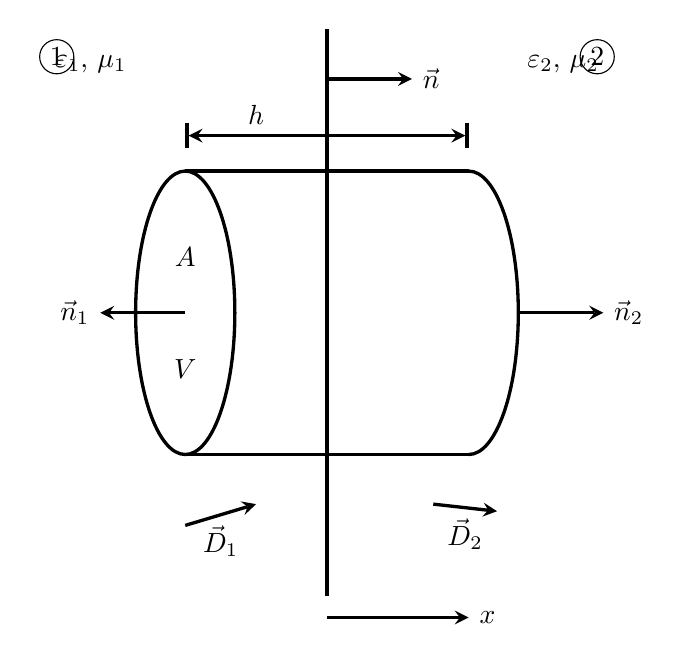
\begin{tikzpicture}[line width = 1.2pt, line join=round,x=1cm,y=1cm,>=stealth, scale = 0.9]
	% Medien und ihre Kennwerte
	\draw (-4.2,4) node [anchor=north west] {\tikz[baseline=(char.base)]{
			\node[shape=circle,draw,inner sep=1.5pt] (char) {1} node [below right=0.4]{$ \varepsilon_1 $, $ \mu_1$}}};
	\draw (4.2,4) node [anchor = north east] {\tikz[baseline=(char.base)]{
			\node[shape=circle,draw,inner sep=1.5pt] (char) {2} node [below left=0.4]{$ \varepsilon_2 $, $ \mu_2$}}};
	% linke Grundfläche
	\draw (-2,0) ellipse (0.7 and 2);
	% Beschriftung der Grundfläche
	\draw (-2,0.5) node [anchor=south] {$ A{} $};
	\draw (-2,-0.5) node [anchor = north] {$ V $};
	% rechte Grundfläche
	\draw (2.7,0) arc (0:90:0.7 and 2);
	\draw (2.7,0) arc (0:-90:0.7 and 2);
	% Mittelachse
	\draw (0,4) -- (0,-4);
	% obere und untere Begrenzung
	\draw (-2,2) -- (2,2);
	\draw (-2,-2) -- (2,-2);
	% Verschiebungsvektoren
	\draw[->] (-2,-3) -- (-1,-2.7) node [midway, below] {$ \vec{D} _1 $};
	\draw[->] (1.5,-2.7) -- (2.4,-2.8) node [midway, below] {$ \vec{D} _2 $};
	% x-Richtung
	\draw [->] (0,-4.3) -- (2,-4.3) node [anchor = west] {$ x $};
	% die Normalen
	\draw [->] (0,3.3) -- (1.2,3.3) node [anchor= west] {$ \vec{n} $};
	\draw [->] (-2,0) -- (-3.2,0) node [anchor = east] {$ \vec{n}_1 $};
	\draw [->] (2.7,0) -- (3.9,0) node [anchor = west] {$ \vec{n}_2 $};
	% Höhe
	\draw [|<->|] (-2,2.5) -- (2,2.5) node [near start, above] {$ h $};
\end{tikzpicture}}
	  \end{center}
	  Es gibt zwei Medien, die Grenzflächen der Dose sind parallel zur Grenzfläche der Medien. Außerdem sind sie klein genug, um $D$ als konstant über diese Fläche anzusehen. Mit \ref{gauss} und \ref{intgauss} folgt das Volumenintegral:
		        $$\iiint\limits_{V}\div \vec{D}\dd V = \iiint\limits_{V}\rho_{\text{V}}\dd V \implies \oiint\limits_{O(V)}\vec{D}\cdot \dd\vec{A}= \iiint\limits_{V}\rho_{\text{V}}\dd V$$ Nun wird der Grenzübergang $h\to0$ ausgeführt. Zum Oberflächenintegral tragen damit nur noch der Deckel und der Boden bei. Da $D$ zudem über die Fläche als konstant angenommen werden kann, ergibt sich das Flächenintegral als Produkt von $\vec{D}$ und der gerichteten Fläche $\vec{A}$. Die Volumenladungsdichte geht durch den Grenzübergang zu einer Flächenladungsdichte über. Auch hier ist die Fläche so klein, dass $\rho_F$ als konstant angenommen werden kann.
		   \begin{equation*}
\begin{split}\left( \vec{n}_{1}\cdot \vec{D}_{1} + \vec{n}_{2}\cdot \vec{D}_{2}\right) A &= \iiint\limits_{V}\rho_{\text{F}}\cdot \delta(x) \dd V = \rho_{\text{F}}\cdot A\\
		       \Rightarrow \left( - \vec{n}\cdot \vec{D}_{1} + \vec{n}\cdot \vec{D}_{2}\right) A &= \iiint\limits_{V}\rho_{\text{F}}\cdot \delta(x) \dd V = \rho_{\text{F}}\cdot A \end{split}   	
		        \end{equation*}
		   \textbf{Die Normalkomponente von $\vec{D}$ ist beim Übergang von Medium 1 auf Medium 2 ggf. unstetig} (Achtung: $\varepsilon$ auf beiden Seiten unterschiedlich):
		        \begin{equation}\label{normD}\begin{split}
				        \boxed{D{}_2^\text{n} - D{}_1^\text{n} = \rho_\text{F} = \vec{n}\cdot \left(\vec{D}_2-\vec{D}_1\right)}
			        \end{split}\end{equation}
		  Diese Formel ist vorzeichenrichtig. Die Normalenvektoren sind immer nach außen orientiert, also ist bei positiver Flächenladung (die Feldrichtung geht auch nach außen) $\vec{n}_1\cdot \vec{D}_1>0$ und $\vec{n}_2\cdot \vec{D}_2>0$. Bei negativer Flächenladung ist dies genau andersherum. Analog folgt aus \ref{quellf}, dass die
		   \textbf{Normalkomponente von $\vec{B}$ immer stetig ist} (Achtung: bei unterschiedlichem $\mu$ springt $H$ dennoch):
		        \begin{equation}\begin{split}\label{normB}
				        \boxed{B{}_2^\text{n} - B{}_1^\text{n} = 0=\vec{n}\cdot\left(\vec{B}_2-\vec{B}_1\right)}
			        \end{split}\end{equation}

  \subsection{Tangentialkomponenten von ${E}$ und ${H}$}
	  \textbf{Stokesche Fläche:}
	  \begin{center}
		  \resizebox{.5\textwidth}{!}{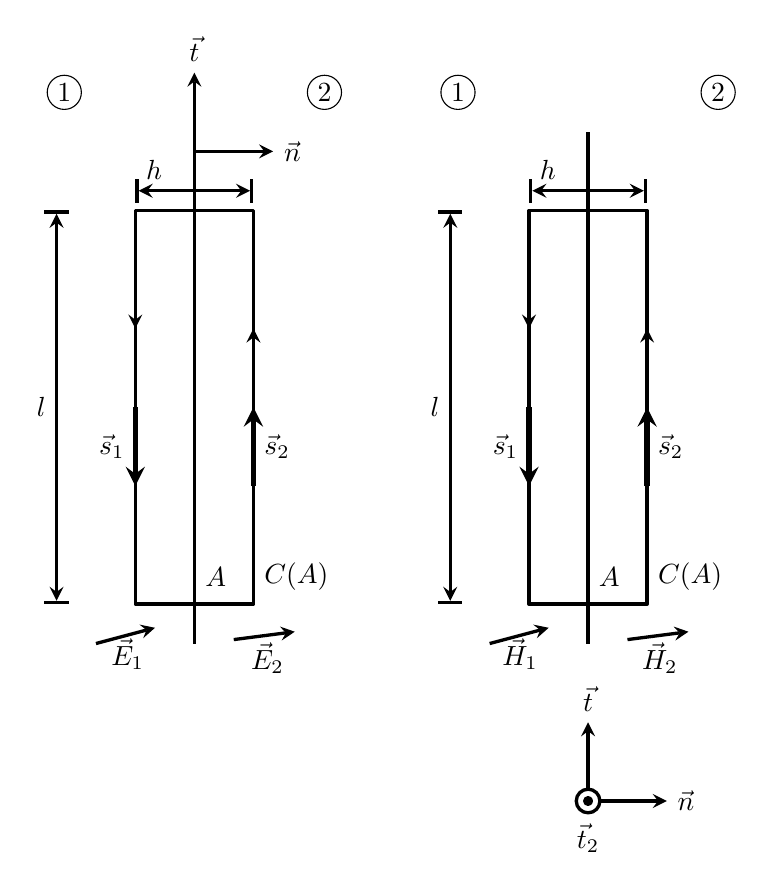
\begin{tikzpicture}[line width = 1.2pt, line join=round,x=0.5cm,y=0.5cm,>=stealth]
	% Mittellinie zeichnen
	\draw (0,-6) -- (0,7);
	% Schleife zeichnen
	\draw (-1.5,-5) rectangle (1.5,5);
	% Richtungen der Schleife
	\draw [->] (-1.5,3) -- (-1.5,2);
	\draw [->] (1.5,1) -- (1.5,2);
	% Vektoren für ds Zeichnen
	\draw [->,line width = 2pt] (-1.5,0) -- (-1.5,-2);
	\draw (-1.5,-1) node[anchor=east] {$\dd \vec{s}_1$};
	\draw [->,line width = 2pt] (1.5,-2) -- (1.5,0);
	\draw (1.5,-1) node[anchor=west] {$\dd \vec{s}_2$};
	% Breite der Schleife
	\draw [|<->|] (1.5,5.5) -- (-1.5,5.5) node[anchor=south west] {$ h $};
	% Höhe der Schleife
	\draw [|<->|] (-3.5,-5) -- (-3.5,5);
	\draw (-3.5,0) node[anchor=east] {$ l $};
	% Normalenvektor
	\draw [->] (0,6.5) -- (2,6.5) node[anchor=west] {$ \vec{n} $};
	% Tangentialvektor
	\draw [->] (0,6.5) -- (0,8.5) node[anchor=south] {$ \vec{t} $};
	% Flächenbezeichnung und Randbezeichnung
	\draw (0,-4.3) node[anchor=west] {$ A $};
	\draw (1.5,-4.3) node[anchor=west] {$ C(A) $};
	% elektrisches Feld
	\draw [->] (-2.5,-6) -- (-1,-5.6) node[anchor=north east] {$ \vec{E}_1 $};
	\draw [->] (1,-5.9) -- (2.55,-5.7) node[anchor=north east] {$ \vec{E}_2 $};
	% Definition der Seiten
	\draw (-4,8) node[anchor=west] {\tikz[baseline=(char.base)]{
			\node[shape=circle,draw,inner sep=1.5pt] (char) {1}}};
	\draw (4,8) node[anchor=east] {\tikz[baseline=(char.base)]{
			\node[shape=circle,draw,inner sep=1.5pt] (char) {2}}};
	% Mittellinie zeichnen
	\draw (10,-6) -- (10,7);
	% Schleife zeichnen
	\draw (8.5,-5) rectangle (11.5,5);
	% Richtungen der Schleife
	\draw [->] (8.5,3) -- (8.5,2);
	\draw [->] (11.5,1) -- (11.5,2);
	% Vektoren für ds Zeichnen
	\draw [->,line width = 2pt] (8.5,0) -- (8.5,-2);
	\draw (8.5,-1) node[anchor=east] {$\dd \vec{s}_1$};
	\draw [->,line width = 2pt] (11.5,-2) -- (11.5,0);
	\draw (11.5,-1) node[anchor=west] {$\dd \vec{s}_2$};
	% Breite der Schleife
	\draw [|<->|] (11.5,5.5) -- (8.5,5.5) node[anchor=south west] {$ h $};
	% Höhe der Schleife
	\draw [|<->|] (6.5,-5) -- (6.5,5);
	\draw (6.5,0) node[anchor=east] {$ l $};
	% Normalenvektor
	\draw [->] (10.3,-10) -- (12,-10) node[anchor=west] {$ \vec{n} $};
	% Tangentialvektor
	\draw [->] (10,-9.7) -- (10,-8) node[anchor=south] {$ \vec{t} $};
	% Tangentialvektor 2
	\draw (10,-10) circle (0.3);
	\filldraw (10,-10) circle (1.2pt);
	\draw (10,-10.3) node[anchor=north] {$ \vec{t}_2 $};
	% Flächenbezeichnung und Randbezeichnung
	\draw (10,-4.3) node[anchor=west] {$ A $};
	\draw (11.5,-4.3) node[anchor=west] {$ C(A) $};
	% magnetisches Feld
	\draw [->] (7.5,-6) -- (9,-5.6) node[anchor=north east] {$ \vec{H} _1 $};
	\draw [->] (11,-5.9) -- (12.55,-5.7) node[anchor=north east] {$ \vec{H} _2 $};
	% Definition der Seiten
	\draw (6,8) node[anchor=west] {\tikz[baseline=(char.base)]{
			\node[shape=circle,draw,inner sep=1.5pt] (char) {1}}};
	\draw (14,8) node[anchor=east] {\tikz[baseline=(char.base)]{
			\node[shape=circle,draw,inner sep=1.5pt] (char) {2}}};
\end{tikzpicture}}
	  \end{center}
		Es gibt zwei Medien mit Grenzfläche. Senkrecht zu dieser Grenzfläche wird eine rechteckförmige Fläche mit Normalenvektor aus der Ebene hinaus gespannt.
		  Mit \ref{ind} und \ref{stokes} folgt das Flächenintegral:
		        $$\iint\limits_{A}\rot \vec{E}\cdot \dd\vec{A}= -\iint\limits_{A}\dfrac{\partial \vec{B} }{\partial t}\cdot \dd\vec{A}\implies\oint\limits_{C(A)}\vec{E}\cdot\dd\vec{s}= -\iint\limits_{A}\dfrac{\partial \vec{B} }{\partial t}\cdot\dd\vec{A}$$
		   Beim Grenzübergang $h\to0$ wird die Flußänderung durch die Fläche verschwinden. Beim Umlaufintegral liefern nur noch die Stücken der Länge $l$ eine Rolle. Also folgt:
		$$-E{}_{1}^{\text{t}}\cdot l + E{}_{2}^{\text{t}}\cdot l = 0$$

		   Daraus folgt, dass die \textbf{Tangentialkomponente von $\vec{E}$ immer stetig ist} (Achtung: Da $\varepsilon$ unterschiedlich ist, kann $D$ dennoch unstetig sein):
		        \begin{equation}\label{tanE}\begin{split}
				        \boxed{E{}_2^\text{t} - E{}_1^\text{t} = 0 \quad \Leftrightarrow \quad \vec{n}\times\left(\vec{{E}}_2-\vec{E}_1\right)=\vec{0}}
			        \end{split}\end{equation}
		   Der Tangentialvektor $\vec{t}$ ist nicht eindeutig. Die Beziehung gilt
		        für alle möglichen Tangentialvektoren $\vec{t}\bot \vec{n}$ \\
			Mit \ref{durchf} folgt analog (Flächenintegral, $h\to 0$, Änderung Verschiebungsstrom = 0):
		        \begin{equation*}\begin{split}
				        -H_{1}^{\text{t}}\cdot l + H_{2}^{\text{t}}\cdot l = \iint\limits_{A}\vec
				        {J}\cdot \dd\vec{A}= \iint\limits_{A}\vec{J}_{\mathrm{A}}\delta(x) \cdot\dd
				        \vec{A}= J_{\mathrm{A}}^{t_2} \cdot l
			        \end{split}\end{equation*}
		 $J_A$ ist hierbei eine Oberflächenstromdichte (siehe auch $\nearrow$ \ref{skin}, die Oberflächenstromdichte ist keine Stromdichte!). \textbf{Die Tangentialkomponente von $\vec{H}$ ist ggf. unstetig:}
		        \begin{equation}\begin{split}\label{tanH}
				        \boxed{H_2^\text{t} - H_1^\text{t} = J_\mathrm{A}^{t_2}\quad \Leftrightarrow \quad \vec{n} \times \left(\vec{H}_2 - \vec{H}_1 \right) =\vec{J}_{A}}
			        \end{split}\end{equation}
		  $J_\mathrm{A}^{t_2}$ bezeichnet die Tangentialkomponente bezüglich des Vektors $\vec{t}_2$. Die Beziehung gilt für alle möglichen Tangentialvektoren mit $\vec{t}_{2}
			        = \vec{n}\times \vec{t} \implies \vec{t}_2\perp\vec{n}$, wobei für $\vec{t}$ nur $\vec{t}\perp\vec{n}$ gelten muss.
		\subsection{Brechungsgesetze}
		\begin{center}
			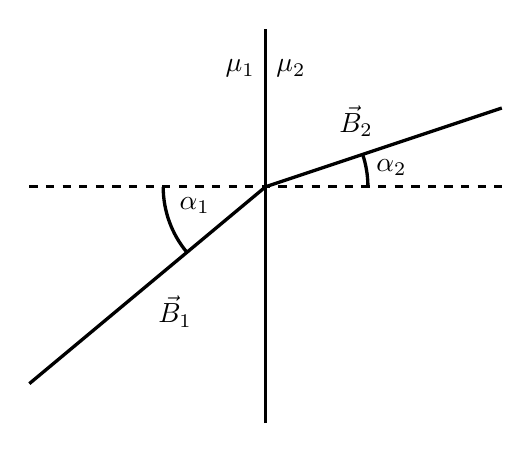
\begin{tikzpicture}[line width = 1.2pt, line join=round,x=1cm,y=1cm,>=stealth]
	% Grenzschicht
	\draw (0,-3) -- (0,2);
	% Referenznormale
	\draw [dashed] (-3,0) -- (3,0);
	% magnetischen Flussdichten
	\draw (-3,-2.5) -- (0,0);
	\draw ({-3/2},{-2.5/2}) node[anchor=north west] {$ \vec{B} _1 $};
	\draw (0,0) -- (3,1);
	\draw ({3/2},{1/2}) node [anchor=south east] {$ \vec{B} _2 $};
	% Winkel
	\draw (-1.3,0) arc (180:220:1.3);
	\draw (-0.9,0) node[anchor=north] {$ \alpha_1 $};
	\draw (1.3,0) arc (0:19:1.3);
	\draw (1.6,0) node[anchor=south] {$ \alpha_2 $};
	% Permeabilität
	\draw (0,1.5) node[anchor=east] {$ \mu_1 $};
	\draw (0,1.5) node[anchor=west] {$ \mu_2 $};
\end{tikzpicture}
		\end{center}
		 Mit \ref{normB} und \ref{tanH} folgt für den Fall $J_\mathrm{A}^{t_2} = 0$ das Brechungsgesetz an Grenzflächen von Stoffen verschiedenen Permeabilitäten:			
		\begin{equation}
			\boxed{\dfrac{\tan \alpha_1}{\tan \alpha_2} = \dfrac{\mu_1}{\mu_2}}
		\end{equation}
		Mit \ref{normD} und \ref{tanE} folgt für den Fall $\rho_\mathrm{F}= 0$ das Brechungsgesetz an Grenzflächen von Stoffen verschiedenen Permittivitäten:	
		\begin{equation}
			\boxed{\dfrac{\tan \alpha_1}{\tan \alpha_2} = \dfrac{\varepsilon_1}{\varepsilon_2}}
		\end{equation}
		Mit \ref{kontstat} und \ref{tanE} folgt für den Fall des stationären Strömungsfeldes das Brechungsgesetz an Grenzflächen von Stoffen mit verschiedenen Leitfähigkeiten:
		\begin{equation}
			\boxed{\dfrac{\tan \alpha_1}{\tan \alpha_2} = \dfrac{\kappa_1}{\kappa_2}}
		\end{equation}
 \section{Einteilung elektromagnetischer Felder}
  Der allgemeine Satz der Maxwell-Gleichungen ist zwar immer korrekt, aber
  \textbf{häufig unnötig kompliziert}. Das Auffinden der Lösungen wird stark vereinfacht,
  wenn \textbf{geeignete Annahmen} gemacht werden. Die vorgestellte Einteilung
  der Vereinfachungen kann auch noch weiter granularisiert werden.\\
  Hier wird die \textbf{Kontinuitätsgleichung} unter dem Querstrich mit angegeben. Außerdem wird durchweg angenommen, dass die \textbf{Flächen zeitunabhängig} sind, also die Differentiation vor das Integral gezogen werden kann.
  \subsection{Keine Einschränkungen - Maxwell-Gleichungen}

	  \begin{align}
		   & \rot \vec{E}= -\dfrac{\partial}{\partial t}\vec{B}          &  & \oint\limits_{C(A)}\vec{E}\cdot \dd\vec{s}= -\dfrac{\dd}{\dd t}\iint\limits_{A}\vec{B}\cdot \dd\vec{A}                                         \\
		   & \rot \vec{H}= \vec{J}+\dfrac{\partial}{\partial t}\vec{D}   &  & \oint\limits_{C(A)}\vec{H}\cdot \dd\vec{s}= \iint\limits_{A}\vec{J}\cdot \dd\vec{A}+ \dfrac{\dd}{\dd t}\iint\limits_{A}\vec{D}\cdot \dd\vec{A} \\
		   & \div \vec{B}= 0                                             &  & \oiint\limits_{O(V)}\vec{B}\cdot \dd\vec{A}= 0                                                                                                 \\
		   & \div \vec{D}= \rho_{\text{V}}                               &  & \oiint\limits_{O(V)}\vec{D}\cdot \dd\vec{A}= \iiint\limits_{V}\rho_{\text{V}}\dd V                                                             \\
		  \nonumber                                                                                                                                                                                         \\
		  \hline
		  \nonumber                                                                                                                                                                                                          \\
		   & \dfrac{\partial \rho_\text{V}}{\partial t}+ \div \vec{J}= 0 &  & \dfrac{\dd}{\dd t}\iiint\limits_{V}\rho_{\text{V}}\dd V + \oiint\limits_{O(V)}\vec{J}\cdot \dd\vec{A}= 0
	  \end{align}
	  Es gibt in der Physik 4 fundamentale Kräfte. Die \textbf{schwachen} und \textbf{starken} \textbf{Kräfte} spielen im Makrokosmos kaum eine Rolle. Die \textbf{Gravitation} spielt nur eine Rolle, wenn sehr große Massen beteiligt sind. Alle anderen Phänomene im Alltag lassen sich mit \textbf{elektromagnetischer} Wechselwirkung erklären, deshalb ist die Lösungsvielfalt so groß.
  \subsection{Statischer Grenzfall $\frac{\partial ...}{\partial t}= 0$}
	  \begin{align}
		   & \rot \vec{E}={\vec{\bm{0}}}          &  & \oint\limits_{C(A)}\vec{E}\cdot \dd\vec{s}={\bm{0}}                                          \\
		   & \rot \vec{H}= \vec{J}+{\vec{\bm{0}}} &  & \oint\limits_{C(A)}\vec{H}\cdot \dd\vec{s}= \iint\limits_{A}\vec{J}\cdot \dd\vec{A}+{\bm{0}} \\
		   & \div \vec{B}= 0                      &  & \oiint\limits_{O(V)}\vec{B}\cdot \dd\vec{A}= 0                                               \\
		   & \div \vec{D}= \rho_{\text{V}}        &  & \oiint\limits_{O(V)}\vec{D}\cdot \dd\vec{A}= \iiint\limits_{V}\rho_{\text{V}}\dd V           \\\nonumber
		  \\
		  \hline
		  \nonumber\\
		   & {\bm{0}}+ \div \vec{J}= 0            &  & {\bm{0}}+ \oiint\limits_{O(V)}\vec{J}\cdot \dd\vec{A}= 0
	  \end{align}
	  Man sieht, dass die elektrischen und die magnetischen Felder im statischen Grenzfall voneinander unabhängig sind. Deswegen unterteilt man in \textbf{Elektrostatik} und \textbf{Magnetostatik}.
	  \subsubsection{Elektrostatik: $J = 0$ }
	  Magnetische Effekte werden ignoriert.\\
		  \textbf{Grundgleichungen der Elektrostatik}
		  \begin{align}
			   & \rot \vec{E}= \vec{0}         &  & \oint\limits_{C(A)}\vec{E}\cdot \dd\vec{s}= 0  \label{GGes1}                                    \\
			   & \div \vec{D}= \rho_{\text{V}} &  & \oiint\limits_{O(V)}\vec{D}\cdot \dd\vec{A}= \iiint\limits_{V}\rho_{\text{V}}\dd V \label{GGes2}
		  \end{align}
		  für \textbf{homogene, lineare, isotrope} Medien ($\vec{D}=\varepsilon_{0}\varepsilon
			  _{r} \vec{E}=\varepsilon \vec{E}$):
		  \begin{align}
			   & \rot \vec{E}= \vec{0}                              &  & \oint\limits_{C(A)}\vec{E}\cdot \dd\vec{s}= 0                                                           \\
			   & \div \vec{E}= \frac{1}{\varepsilon}\rho_{\text{V}} &  & \oiint\limits_{O(V)}\vec{E}\cdot \dd\vec{A}= \frac{1}{\varepsilon}\iiint\limits_{V}\rho_{\text{V}}\dd V
		  \end{align}
		  \textbf{Poisson-Gleichung} (Elektrisches Feld ist wirbelfrei $\nearrow$ \ref{poin1}):
		  \begin{equation}
		  	 \rot \vec{E}= \vec{0}\Rightarrow \vec{E}= -\grad \phi \to -\div \vec{E}= \div
		  	\grad \phi = \bm{\Delta\phi = - \frac{1}{\varepsilon}\rho_\text{V}}
		  \end{equation}
		  Siehe auch \ref{es}.
  \subsubsection{Magnetostatik: $\rho_{\mathrm{V}}= 0$}
Elektrische Effekte werden ignoriert.\\
	  \textbf{Grundgleichungen der Magnetostatik}

	  \begin{align}
		   & \rot \vec{H}= \vec{J} &  & \oint\limits_{C(A)}\vec{H}\cdot \dd\vec{s}= \iint\limits_{A}\vec{J}\cdot \dd\vec{A} \label{GGms1} \\
		   & \div \vec{B}= 0       &  & \oiint\limits_{O(V)}\vec{B}\cdot \dd\vec{A}= 0                                   \label{GGms2}   \\
		   & \div \vec{J}= 0       &  & \oiint\limits_{O(V)}\vec{J}\cdot \dd\vec{A}= 0
	  \end{align}

	  für \textbf{homogene, lineare, isotrope} Medien ($\vec{B}=\mu_{0}\mu_{r} \vec{H}
		  =\mu \vec{H}$):

	  \begin{align}
		   & \rot \vec{B}= \mu\vec{J} &  & \oint\limits_{C(A)}\vec{B}\cdot \dd\vec{s}= \mu\iint\limits_{A}\vec{J}\cdot \dd\vec{A} \\
		   & \div \vec{B}= 0          &  & \oiint\limits_{O(V)}\vec{B}\cdot \dd\vec{A}= 0
	  \end{align}
	  Folgendes führt später zur \textbf{Eichung} (B-Feld ist divergenzfrei $\nearrow$ \ref{poin2}):
\begin{equation}
		  \div \vec{B}= 0 \Rightarrow \vec{B}= \rot \vec{A}\to \rot \vec{B}= \textbf{rot rot}\vec{\bm{A}}= \bm{\mu}\vec{\bm{J}}\end{equation} 
		  Siehe auch \ref{ms}.
	  \subsubsection{Stationäres Strömungsfeld: $\mathrm{div}{J}= 0$}
	   Die \textbf{Grundgleichungen des Stationären Strömungsfeldes} in Gebieten \textit{ohne Urspannung} ($\nearrow$ \ref{Urspannung}) sind:
		  { \begin{align}&\rot \vec{E}= \vec{0}&&\oint\limits_{C(A)}\vec{E}\cdot \dd\vec{s}= 0\label{GGstatstr1}\\&\rot \vec{H}= \vec{J}&&\oint\limits_{C(A)}\vec{H}\cdot \dd\vec{s}= \iint\limits_{A}\vec{J}\cdot \dd\vec{A}\\&0=\div \vec{J}\stackrel{\kappa\neq f(\vec{r})}{=} \kappa\div \vec{E}&&\oiint\limits_{O(V)}\vec{J}\cdot \dd\vec{A}= \oiint\limits_{O(V)}\kappa\vec{E}\cdot \dd\vec{A}= 0\label{GGstatstr3}\end{align} }
			   Siehe auch \ref{statstr}.

  \subsection{Quasistationäres Feld}
		   Es sind zeitliche Änderungen vorhanden; diese sind aber \enquote{langsam}, d.h. die Momentanaufnahmen der Felder entsprechen den statischen Feldern.
		   In dem betrachteten Gebiet müssen dafür die Wirkungen \enquote{verzögerungsfrei} übermittelt werden $\to$ Keine \textbf{Retardierung} (z.B. ist optisches Signal näherungsweise instantan, der Schall ist langsam $\to$ nur wenn Gebiet klein genug ist braucht nicht retardiert zu werden). Außerdem gibt es keine Abstrahlung,
		   Orts- und Zeitabhängigkeit sind entkoppelt und Berechnungen sind mit den Lösungsmethoden der Statik (aber zeitabhängig) möglich. Man unterscheidet zwei Fälle:
		        \begin{enumerate}
			        \item Quasi-Elektrostatik (Induktion vernachlässigen)
			              \begin{equation}\begin{split}
					              \dfrac{\partial}{\partial t}\vec{D}\neq \vec{0}\text{ und }\dfrac{\partial}
					              {\partial t}\vec{B}\to \vec{0}\Rightarrow \rot \vec{E}\to \vec{0}
				              \end{split}\end{equation}

			        \item Quasi-Magnetostatik (Verschiebungsstrom vernachlässigen)
			              \begin{equation}\begin{split}
					              \dfrac{\partial}{\partial t}\vec{D}\to \vec{0}\text{ und }\dfrac{\partial}
					              {\partial t}\vec{B}\neq \vec{0}\Rightarrow \rot \vec{H}\to \vec{J}
				              \end{split}\end{equation}
		        \end{enumerate}
	  \subsubsection{Quasi-Elektrostatik}
		  \begin{align}
			   & \textbf{rot}\vec{\bm{E}}= \vec{\bm{0}}                      &  & \oint\limits_{\bm{C(A)}}\vec{\bm{E}}\cdot \textbf{d}\vec{\bm{s}}= \bm{0}                                                                       \\
			   & \rot \vec{H}= \vec{J}+\dfrac{\partial}{\partial t}\vec{D}   &  & \oint\limits_{C(A)}\vec{H}\cdot \dd\vec{s}= \iint\limits_{A}\vec{J}\cdot \dd\vec{A}+ \dfrac{\dd}{\dd t}\iint\limits_{A}\vec{D}\cdot \dd\vec{A} \\
			   & \div \vec{B}= 0                                             &  & \oiint\limits_{O(V)}\vec{B}\cdot \dd\vec{A}= 0                                                                                                 \\
			   & \div \vec{D}= \rho_{\text{V}}                               &  & \oiint\limits_{O(V)}\vec{D}\cdot \dd\vec{A}= \iiint\limits_{V}\rho_{\text{V}}\dd V                                                             \\
			  \nonumber                                                                                                                                                                                                          \\
			  \hline
			  \nonumber                                                                                                                                                                                                          \\
			   & \dfrac{\partial \rho_\text{V}}{\partial t}+ \div \vec{J}= 0 &  & \dfrac{\dd}{\dd t}\iiint\limits_{V}\rho_{\text{V}}\dd V + \oiint\limits_{O(V)}\vec{J}\cdot \dd\vec{A}= 0
		  \end{align}
		  Siehe auch \ref{eqs}.
	  \subsubsection{Quasi-Magnetostatik}
		  \begin{align}
			   & \rot \vec{E}= -\dfrac{\partial}{\partial t}\vec{B}          &  & \oint\limits_{C(A)}\vec{E}\cdot \dd\vec{s}= -\dfrac{\dd}{\dd t}\iint\limits_{A}\vec{B}\cdot \dd\vec{A}                                  \\
			   & {\textbf{rot} \vec{\bm{H}} = \vec{\bm{J}}}                  &  & {\oint\limits_{\bm{C(A)}} \vec{\bm{H}} \cdot \textbf{d}\vec{\bm{s}} = \iint\limits_{\bm{A}} \vec{\bm{J}} \cdot \textbf{d}\vec{\bm{A}} } \\
			   & \div \vec{B}= 0                                             &  & \oiint\limits_{O(V)}\vec{B}\cdot \dd\vec{A}= 0                                                                                          \\
			   & \div \vec{D}= \rho_{\text{V}}                               &  & \oiint\limits_{O(V)}\vec{D}\cdot \dd\vec{A}= \iiint\limits_{V}\rho_{\text{V}}\dd V                                                      \\
			  \nonumber                                                                                                                                                                                                   \\
			  \hline
			  \nonumber                                                                                                                                                                                                   \\
			   & \dfrac{\partial \rho_\text{V}}{\partial t}+ \div \vec{J}= 0 &  & \dfrac{\dd}{\dd t}\iiint\limits_{V}\rho_{\text{V}}\dd V + \oiint\limits_{O(V)}\vec{J}\cdot \dd\vec{A}= 0
		  \end{align}
		  Siehe auch \ref{mqs}.